\documentclass[12pt,a4paper]{report}

\usepackage{fontspec}
\usepackage{polyglossia}
\setmainlanguage{russian}
\setotherlanguage{english}
\setmainfont{Times New Roman}
\setsansfont{Arial}
\setmonofont{Consolas}

\newfontfamily\cyrillicfont{Times New Roman}
\newfontfamily\cyrillicfontsf{Arial}
\newfontfamily\cyrillicfonttt{Consolas}
\usepackage{geometry}
\geometry{left=30mm,right=15mm,top=20mm,bottom=20mm}
\usepackage{setspace}
\onehalfspacing
\usepackage{indentfirst}
\setlength{\parindent}{1.25cm}
\usepackage{graphicx}
\graphicspath{{../results/}{figures/}}
\usepackage{booktabs}
\usepackage{longtable}
\usepackage{array}
\usepackage{amsmath}
\usepackage{listings}
\usepackage{xcolor}
\usepackage{hyperref}
\hypersetup{
  colorlinks=true,
  linkcolor=black,
  citecolor=black,
  urlcolor=blue,
  pdftitle={Курсовая работа: адаптивная оркестрация многоагентных LLM-систем},
  pdfauthor={almazgde}
}

\lstdefinestyle{code}{
  basicstyle=\ttfamily\small,
  breaklines=true,
  frame=single,
  columns=fullflexible,
  showstringspaces=false,
  keywordstyle=\color{blue!60!black},
  commentstyle=\color{green!40!black}
}
\lstset{style=code}

\newcommand{\code}[1]{\texttt{#1}}
\newcommand{\project}{\code{adaptive-mas-coursework}}

\begin{document}

\begin{titlepage}
\begin{center}
Министерство науки и высшего образования Российской Федерации\\
Образовательная организация\\[2cm]

\textbf{КУРСОВАЯ РАБОТА}\\[0.5cm]
по дисциплине: программная инженерия и интеллектуальные системы\\[1cm]

\textbf{Исследование адаптивной оркестрации многоагентных LLM-систем на основе графов зависимостей задач}\\[2cm]
\end{center}

\begin{flushright}
Выполнил: студент\\
Проверил: преподаватель\\
\end{flushright}

\vfill
\begin{center}
2026
\end{center}
\end{titlepage}

\tableofcontents
\clearpage

\chapter*{Введение}
\addcontentsline{toc}{chapter}{Введение}

Современные LLM-системы всё чаще строятся не как одиночный вызов языковой модели, а как композиция нескольких специализированных агентов. Один агент может планировать, другой выполнять исследование, третий проверять результат, а финальный компонент синтезировать ответ. Такая архитектура повышает выразительность системы, но создаёт новую инженерную задачу: необходимо выбрать порядок и топологию исполнения подзадач.

Актуальность работы связана с тем, что простая последовательная оркестрация плохо использует независимость подзадач, а наивный параллелизм может добавлять лишние накладные расходы. Для реалистичного сравнения topology strategies недостаточно измерять только latency: необходимо учитывать стоимость узлов, critical path, качество результата и устойчивость к отказам.

Цель работы --- разработать и исследовать прототип адаптивной оркестрации многоагентных LLM-систем, в котором задача представляется DAG-графом, а топология исполнения выбирается на основе структурных, стоимостных и экспериментально полученных признаков.

Для достижения цели были поставлены следующие задачи:
\begin{enumerate}
  \item реализовать модель DAG с узлами, рёбрами и зависимостями;
  \item реализовать structural и weighted graph metrics;
  \item реализовать static и adaptive topology selectors;
  \item добавить cost-aware и learned adaptive selection;
  \item реализовать execution layer с mock agents и tracing;
  \item добавить quality evaluation и failure simulation;
  \item построить benchmark runner, CLI и конфигурации экспериментов;
  \item проверить проект unit tests и reproducibility checks;
  \item оформить результаты в виде CSV, графиков и timeline visualization.
\end{enumerate}

Объект исследования --- многоагентные LLM-системы, исполняющие сложные задачи как набор зависимых подзадач.

Предмет исследования --- методы выбора topology execution strategy для DAG-задач с учётом latency, cost, quality и robustness.

Методы исследования включают моделирование DAG, анализ критического пути, synthetic benchmarks, эвристический scoring, lightweight nearest-neighbor learned baseline, unit testing и анализ execution traces.

Практическая значимость работы состоит в создании воспроизводимого прототипа \project{}, который позволяет сравнивать orchestration strategies локально без внешних API, сохранять результаты в CSV и строить визуализации для анализа расписания выполнения DAG.

\chapter{Теоретические основы}

\section{Многоагентные LLM-системы}

Многоагентная LLM-система представляет собой программную архитектуру, в которой сложная задача распределяется между несколькими агентами. Общие принципы анализа multi-agent systems описаны в классической литературе по многоагентным системам~\cite{wooldridge2009multiagent}. В реальных системах агенты могут обращаться к языковой модели, инструментам поиска, базам знаний или внешним API. В реализованном проекте используются mock agents, поэтому исследование сфокусировано на orchestration layer, а не на качестве конкретного LLM backend.

Основное преимущество многоагентного подхода заключается в декомпозиции: разные шаги могут выполняться независимо или частично параллельно. Однако это преимущество проявляется только при корректном управлении зависимостями.

\section{DAG-графы задач}

Задача моделируется направленным ациклическим графом \(G=(V,E)\), где \(V\) --- множество подзадач, а \(E\) --- зависимости между ними. Ребро \(u \rightarrow v\) означает, что узел \(v\) может быть выполнен только после завершения узла \(u\). Ацикличность важна, потому что цикл зависимостей привёл бы к невозможности построить корректный порядок исполнения.

Для DAG существует топологическая сортировка. Она задаёт допустимый порядок исполнения узлов и служит основой для sequential, parallel, hierarchical и hybrid executors. Алгоритмическая база топологической сортировки и работы с графами опирается на стандартные методы анализа графов~\cite{kahn1962topological,cormen2009algorithms}.

\section{Topology execution strategies}

В проекте рассматриваются четыре базовые топологии:

\begin{table}[h]
\centering
\caption{Topology execution strategies}
\begin{tabular}{p{0.22\textwidth}p{0.68\textwidth}}
\toprule
Topology & Описание \\
\midrule
\code{sequential} & Узлы исполняются по одному в топологическом порядке; overhead минимален, параллелизм не используется. \\
\code{parallel} & На каждом шаге запускаются все готовые узлы, зависимости которых выполнены. \\
\code{hierarchical} & Исполнение организуется через coordinator/aggregate pattern с дополнительными координационными затратами. \\
\code{hybrid} & Граф исполняется слоями: внутри слоя возможен параллелизм, между слоями сохраняется порядок. \\
\bottomrule
\end{tabular}
\end{table}

\section{Critical path и weighted critical path}

Critical path --- самый длинный путь зависимостей в DAG. Он задаёт нижнюю границу времени исполнения: узлы на одном пути не могут быть выполнены параллельно относительно друг друга. Идея critical path широко используется в планировании и управлении проектами~\cite{kerzner2017project}.

В weighted DAG каждому узлу \(v\) сопоставляется стоимость \(c(v)\). В проекте она берётся из \code{node.data["cost"]}, а если стоимость не задана, используется безопасное значение по умолчанию \code{DEFAULT\_NODE\_COST = 0.1}. Weighted critical path определяется как:

\[
WCP(G)=\max_{p \in Paths(G)} \sum_{v \in p} c(v).
\]

Эта метрика точнее обычной длины пути, потому что учитывает неоднородность узлов: короткий путь из дорогих задач может сильнее влиять на latency, чем длинный путь из дешёвых задач.

\section{Trade-off latency, cost, quality и robustness}

Выбор topology является многокритериальной задачей. Parallel execution может снижать latency, но увеличивать coordination overhead. Fallback logic может повышать success rate, но ухудшать consistency score. Learned selector может повторять удачные решения из synthetic benchmark data, но его качество зависит от training set и objective score.

В работе используются следующие группы метрик:
\begin{enumerate}
  \item latency и execution cost;
  \item structural и weighted graph metrics;
  \item quality metrics;
  \item robustness metrics;
  \item selected topology и selector mode.
\end{enumerate}

\chapter{Проектирование и архитектура системы}

\section{Общая архитектура}

Проект \project{} организован как набор модулей Python и использует \code{networkx.DiGraph} как базовую структуру для DAG~\cite{networkx,projectrepo}. Архитектура показана на рисунке~\ref{fig:architecture}.

\begin{figure}[h]
\centering
\fbox{\begin{minipage}{0.92\textwidth}
\centering
\begin{tabular}{c}
\code{configs/}, \code{run.py}, CLI commands \\
\(\downarrow\) \\
\code{experiments.benchmarks}: synthetic graphs, runner, CSV output \\
\(\downarrow\) \\
\code{adaptive\_mas.dag} + \code{adaptive\_mas.metrics} \\
\(\downarrow\) \\
\code{adaptive\_mas.topology}: static, rule-based, cost-aware, learned selectors \\
\(\downarrow\) \\
\code{adaptive\_mas.execution} + \code{adaptive\_mas.agents} \\
\(\downarrow\) \\
\code{adaptive\_mas.evaluation}: quality and robustness \\
\(\downarrow\) \\
\code{results/}: CSV, JSON traces, PNG plots, learned model
\end{tabular}
\end{minipage}}
\caption{Архитектурная схема проекта}
\label{fig:architecture}
\end{figure}

\section{Модули проекта}

\begin{longtable}{p{0.30\textwidth}p{0.60\textwidth}}
\caption{Реальные модули проекта}\\
\toprule
Модуль & Назначение \\
\midrule
\endfirsthead
\toprule
Модуль & Назначение \\
\midrule
\endhead
\code{adaptive\_mas.dag} & Node, Edge, DAG, зависимости и топологическая сортировка. \\
\code{adaptive\_mas.metrics} & Structural metrics, weighted metrics, critical path и weighted critical path. \\
\code{adaptive\_mas.topology} & TopologyType, rule-based selector, cost-aware selector, learned selector. \\
\code{adaptive\_mas.execution} & Sequential, parallel, hierarchical и hybrid executors, execution traces, failure handling. \\
\code{adaptive\_mas.agents} & Mock agents, имитирующие выполнение ролей без real LLM API. \\
\code{adaptive\_mas.evaluation} & Heuristic quality evaluation и robustness metrics. \\
\code{experiments.benchmarks} & Synthetic graph factory и benchmark runner. \\
\code{run.py} & Единый CLI для demo, benchmark, visualization, experiments и training learned selector. \\
\code{configs/} & JSON-конфигурации экспериментов. \\
\code{results/} & CSV, PNG, JSON traces и learned selector model. \\
\bottomrule
\end{longtable}

\section{DAG execution pipeline}

\begin{figure}[h]
\centering
\fbox{\begin{minipage}{0.9\textwidth}
\centering
\code{Synthetic DAG} \(\rightarrow\)
\code{GraphMetrics} \(\rightarrow\)
\code{TopologySelector} \(\rightarrow\)
\code{Executor} \(\rightarrow\)
\code{Trace} \(\rightarrow\)
\code{Quality/Robustness} \(\rightarrow\)
\code{CSV/PNG}
\end{minipage}}
\caption{Pipeline исполнения DAG-задачи}
\label{fig:pipeline}
\end{figure}

\chapter{Реализация}

\section{Node, Edge и DAG}

Классы \code{Node}, \code{Edge} и \code{DAG} находятся в \code{adaptive\_mas.dag}. Узел хранит идентификатор, task, agent и произвольные данные, включая возможную стоимость \code{node.data["cost"]}. Рёбра описывают зависимости. DAG предоставляет методы добавления узлов и рёбер, проверки ацикличности, получения predecessors/successors и топологической сортировки.

\section{GraphMetrics и weighted metrics}

\code{GraphMetrics} рассчитывает depth, density, parallel width, max degree и critical path length. В финальной версии добавлены weighted metrics:

\begin{enumerate}
  \item \code{node\_cost(node\_id)};
  \item \code{total\_node\_cost()};
  \item \code{average\_node\_cost()};
  \item \code{max\_node\_cost()};
  \item \code{cost\_variance()};
  \item \code{weighted\_critical\_path\_length()};
  \item \code{weighted\_parallel\_width()}.
\end{enumerate}

Если стоимость узла отсутствует, используется default mock execution cost. Метрики безопасно обрабатывают пустой DAG.

\section{Topology selectors}

Rule-based adaptive selector выбирает topology по структурным эвристикам: глубина, ширина, плотность и max degree. Cost-aware selector оценивает все поддерживаемые топологии и использует простую интерпретируемую формулу:

\[
score = expected\ latency + coordination\ overhead + critical\ path\ penalty.
\]

Learned adaptive selector реализован в \code{adaptive\_mas.topology.learned\_selector}. Это lightweight nearest-neighbor baseline без тяжёлых ML-зависимостей. Feature vector включает node count, edge count, graph depth, density, parallel width, max degree, total node cost, average node cost, max node cost, weighted critical path и weighted parallel width.

Training objective documented in the model file:
\[
objective\_score = estimated\_latency\_with\_overhead + 0.05 \cdot execution\_cost.
\]

\section{Executors и mock agents}

В execution layer реализованы \code{SequentialExecutor}, \code{ParallelExecutor}, \code{HierarchicalExecutor} и \code{HybridExecutor}. Executors собирают execution trace: \code{node\_id}, task, agent, start time, end time, duration, topology, status, retry count и fallback flags.

Mock agents имитируют роли planner, researcher, critic и synthesizer. Они не обращаются к LLM API, что делает эксперименты быстрыми и воспроизводимыми.

\section{Quality и robustness evaluation}

\code{QualityEvaluator} реализует deterministic heuristic model. Он оценивает completeness, consistency, synthesis, dependency coverage и overall quality. Failed, skipped и fallback nodes снижают соответствующие scores.

Robustness evaluation считает success rate, failed node count, skipped node count, retry count total, fallback count, recovery success rate и wasted work estimate. Failure simulation поддерживает synthetic exception, timeout и empty result.

\section{Benchmark runner, CLI и visualization}

Benchmark runner генерирует synthetic graphs, запускает стратегии и сохраняет результаты в CSV. CLI \code{run.py} поддерживает команды \code{demo}, \code{benchmark}, \code{visualize}, \code{experiment} и \code{train-selector}. Timeline visualization строит Gantt chart из execution trace и сохраняет PNG в \code{results/}.

\chapter{Экспериментальное исследование}

\section{Synthetic graph scenarios}

В финальном benchmark использованы четыре сценария:

\begin{enumerate}
  \item \code{wide\_sparse};
  \item \code{deep\_dependency};
  \item \code{layered};
  \item \code{centralized\_coordinator}.
\end{enumerate}

Они покрывают широкий параллелизм, глубокие зависимости, послойную структуру и coordinator pattern.

\section{Сравниваемые стратегии}

\begin{table}[h]
\centering
\caption{Selector modes}
\begin{tabular}{p{0.30\textwidth}p{0.58\textwidth}}
\toprule
Mode & Смысл \\
\midrule
\code{static} & Исполняется явно заданная topology: sequential, parallel, hierarchical или hybrid. \\
\code{rule\_based\_adaptive} & Выбор topology по structural graph metrics. \\
\code{cost\_aware\_adaptive} & Выбор topology по latency, overhead и critical path penalty. \\
\code{learned\_adaptive} & Nearest-neighbor baseline, обученный на synthetic benchmark data. \\
\bottomrule
\end{tabular}
\end{table}

\section{Benchmark methodology}

Финальный запуск был выполнен командой:

\begin{lstlisting}
python run.py benchmark --selector all --model results/learned_selector_model.json --runs 10
\end{lstlisting}

Перед этим learned selector был обучен:

\begin{lstlisting}
python run.py train-selector --runs 100 --output results/learned_selector_model.json
\end{lstlisting}

Результаты сохранены в \code{results/benchmark\_results.csv} и \code{results/benchmark\_summary.csv}. Файл \code{results/experiment\_config\_used.json} фиксирует использованную конфигурацию. Unit tests запускались командой:

\begin{lstlisting}
$env:PYTHONDONTWRITEBYTECODE='1'; python -m unittest discover -s tests
\end{lstlisting}

Фактический результат тестирования: 56 тестов, статус OK.

\section{Collected metrics}

\begin{longtable}{p{0.32\textwidth}p{0.58\textwidth}}
\caption{Основные метрики benchmark}\\
\toprule
Метрика & Описание \\
\midrule
\endfirsthead
\toprule
Метрика & Описание \\
\midrule
\endhead
\code{latency} & Итоговая задержка исполнения DAG. \\
\code{cost} & Synthetic execution cost. \\
\code{coordination\_overhead} & Накладные расходы координации. \\
\code{parallel\_efficiency} & Эффективность относительно critical path. \\
\code{weighted\_critical\_path} & Максимальная суммарная стоимость пути в DAG. \\
\code{weighted\_parallel\_width} & Максимальная суммарная стоимость одного уровня. \\
\code{overall\_quality\_score} & Итоговая heuristic quality score. \\
\code{success\_rate} & Доля успешно выполненных узлов. \\
\code{selector\_mode} & Static, rule-based, cost-aware или learned adaptive. \\
\code{selected\_topology} & Фактически выбранная topology. \\
\bottomrule
\end{longtable}

\chapter{Анализ результатов}

\section{Benchmark summary}

В таблице~\ref{tab:summary} приведены агрегированные результаты из фактического файла \code{results/benchmark\_summary.csv}, сформированного финальным запуском. Все значения являются результатом текущего состояния репозитория; при изменении seed, числа runs или реализации они должны пересчитываться.

\begin{longtable}{p{0.25\textwidth}p{0.22\textwidth}p{0.16\textwidth}r r r}
\caption{Benchmark summary из \code{results/benchmark\_summary.csv}}
\label{tab:summary}\\
\toprule
Graph type & Mode & Topology & Runs & Avg latency & Avg cost \\
\midrule
\endfirsthead
\toprule
Graph type & Mode & Topology & Runs & Avg latency & Avg cost \\
\midrule
\endhead
\code{centralized\_coordinator} & cost-aware & parallel & 10 & 1.119 & 4.100 \\
\code{centralized\_coordinator} & learned & parallel & 10 & 1.119 & 4.100 \\
\code{centralized\_coordinator} & rule-based & hierarchical & 10 & 1.238 & 3.984 \\
\code{centralized\_coordinator} & static & hierarchical & 10 & 1.238 & 3.984 \\
\code{centralized\_coordinator} & static & hybrid & 10 & 1.265 & 3.959 \\
\code{centralized\_coordinator} & static & parallel & 10 & 1.119 & 4.100 \\
\code{centralized\_coordinator} & static & sequential & 10 & 3.701 & 3.666 \\
\code{deep\_dependency} & cost-aware & sequential & 10 & 3.697 & 3.664 \\
\code{deep\_dependency} & learned & sequential & 10 & 3.697 & 3.664 \\
\code{deep\_dependency} & rule-based & sequential & 10 & 3.697 & 3.664 \\
\code{deep\_dependency} & static & hierarchical & 10 & 4.158 & 4.213 \\
\code{deep\_dependency} & static & hybrid & 10 & 4.053 & 4.031 \\
\code{deep\_dependency} & static & parallel & 10 & 3.869 & 3.971 \\
\code{deep\_dependency} & static & sequential & 10 & 3.697 & 3.664 \\
\code{layered} & cost-aware & parallel & 10 & 0.919 & 3.928 \\
\code{layered} & learned & parallel & 10 & 0.919 & 3.928 \\
\code{layered} & rule-based & hybrid & 10 & 1.154 & 3.929 \\
\code{layered} & static & hierarchical & 10 & 1.207 & 4.036 \\
\code{layered} & static & hybrid & 10 & 1.154 & 3.929 \\
\code{layered} & static & parallel & 10 & 0.919 & 3.928 \\
\code{layered} & static & sequential & 10 & 3.700 & 3.665 \\
\code{wide\_sparse} & cost-aware & parallel & 10 & 1.257 & 4.045 \\
\code{wide\_sparse} & learned & parallel & 10 & 1.257 & 4.045 \\
\code{wide\_sparse} & rule-based & parallel & 10 & 1.257 & 4.045 \\
\code{wide\_sparse} & static & hierarchical & 10 & 1.397 & 3.991 \\
\code{wide\_sparse} & static & hybrid & 10 & 1.377 & 3.920 \\
\code{wide\_sparse} & static & parallel & 10 & 1.257 & 4.045 \\
\code{wide\_sparse} & static & sequential & 10 & 3.683 & 3.655 \\
\bottomrule
\end{longtable}

\section{Comparison of topology strategies}

Если агрегировать только static strategies по четырём graph types, текущий CSV даёт значения из таблицы~\ref{tab:staticavg}. Эти числа показывают, что в synthetic setup parallel имеет меньшую среднюю latency, чем другие static режимы, но также имеет более высокую среднюю стоимость, чем sequential. Это не доказывает универсальное превосходство parallel topology, потому что результаты зависят от набора synthetic graphs и mock cost model.

\begin{table}[h]
\centering
\caption{Средние значения static topologies по четырём graph types}
\label{tab:staticavg}
\begin{tabular}{lrrr}
\toprule
Topology & Avg latency & Avg cost & Avg efficiency \\
\midrule
hierarchical & 2.000 & 4.056 & 0.633 \\
hybrid & 1.962 & 3.960 & 0.640 \\
parallel & 1.791 & 4.011 & 0.729 \\
sequential & 3.695 & 3.663 & 0.387 \\
\bottomrule
\end{tabular}
\end{table}

\section{Comparison of selector modes}

\begin{table}[h]
\centering
\caption{Средние значения selector modes по текущему benchmark summary}
\label{tab:selectormodes}
\begin{tabular}{lrrrr}
\toprule
Mode & Groups & Avg latency & Avg cost & Avg quality \\
\midrule
cost-aware adaptive & 4 & 1.748 & 3.934 & 0.900 \\
learned adaptive & 4 & 1.748 & 3.934 & 0.900 \\
rule-based adaptive & 4 & 1.836 & 3.905 & 0.900 \\
static & 16 & 2.362 & 3.922 & 0.900 \\
\bottomrule
\end{tabular}
\end{table}

В текущем финальном запуске cost-aware и learned selectors выбрали одинаковые topology для всех четырёх graph categories. Это является фактическим наблюдением по сохранённому CSV, но не означает, что learned selector всегда будет совпадать с cost-aware selector или превосходить другие режимы. Learned selector обучен на synthetic benchmark data и является baseline.

\section{Визуализации}

Файлы визуализаций находятся в \code{results/}. В работу включены реальные PNG, созданные проектом.

\begin{figure}[h]
\centering
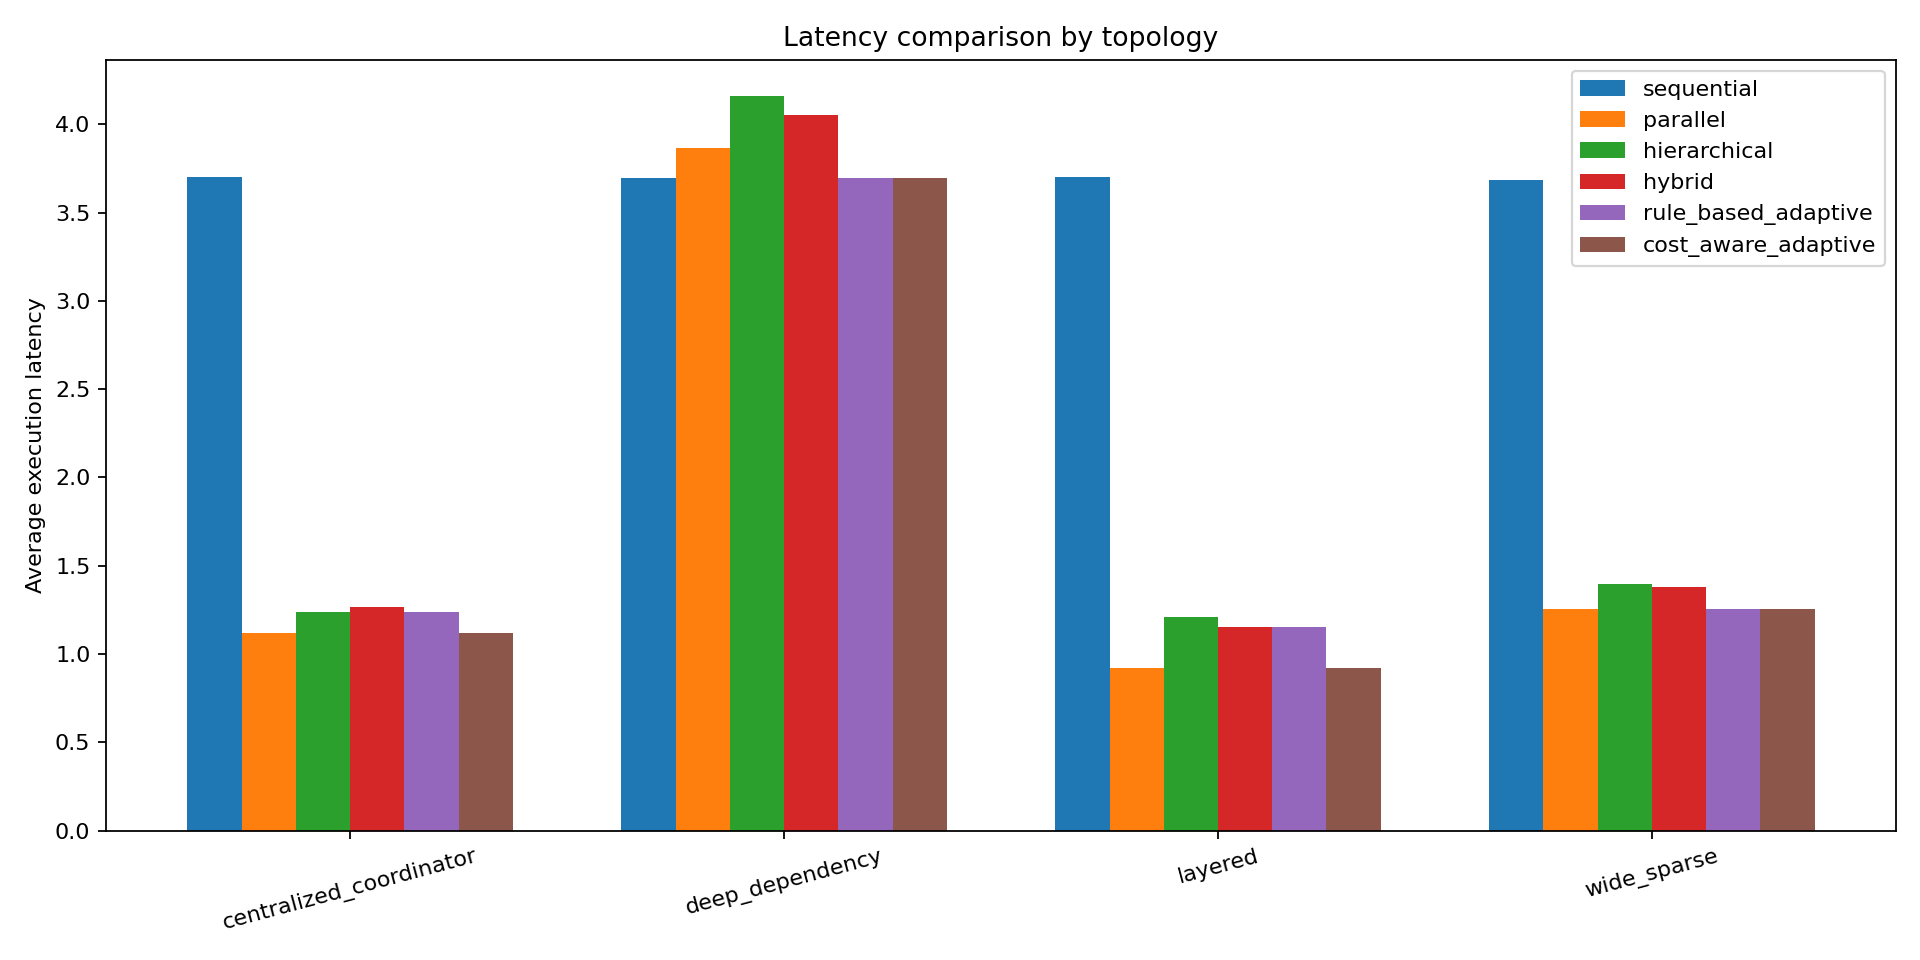
\includegraphics[width=0.86\textwidth]{latency_comparison.png}
\caption{Сравнение latency по graph type и topology}
\label{fig:latency}
\end{figure}

\begin{figure}[h]
\centering
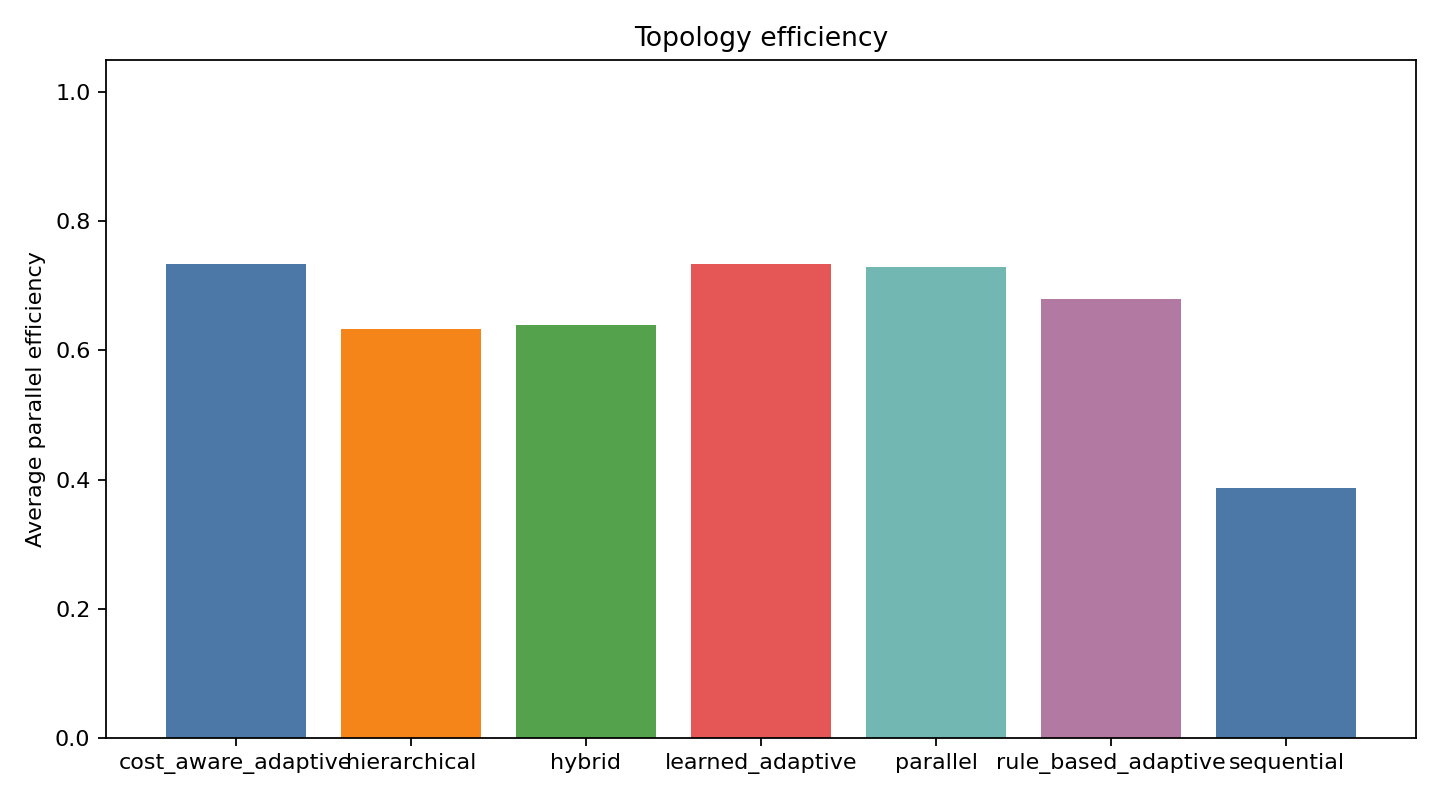
\includegraphics[width=0.86\textwidth]{topology_efficiency.png}
\caption{Parallel efficiency topology strategies}
\label{fig:efficiency}
\end{figure}

\begin{figure}[h]
\centering
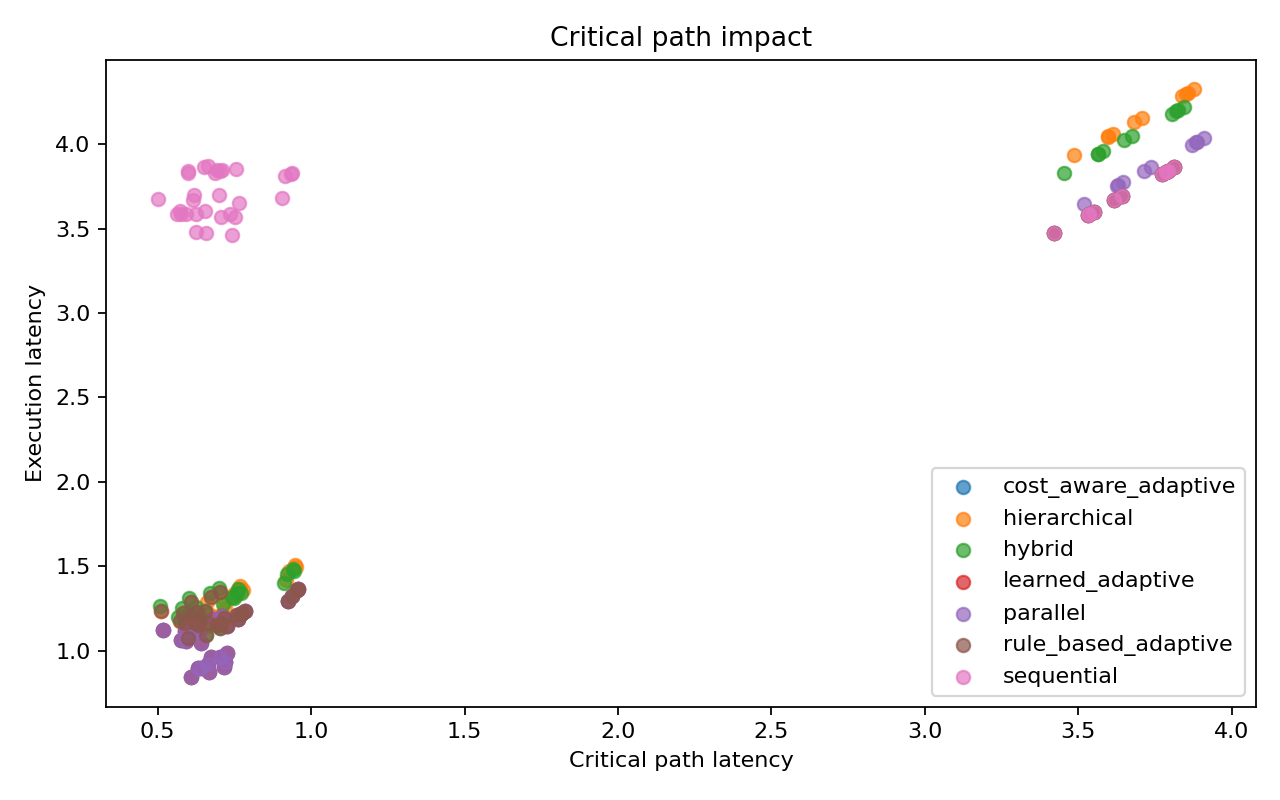
\includegraphics[width=0.86\textwidth]{critical_path_impact.png}
\caption{Влияние critical path latency на total latency}
\label{fig:criticalpath}
\end{figure}

\begin{figure}[h]
\centering
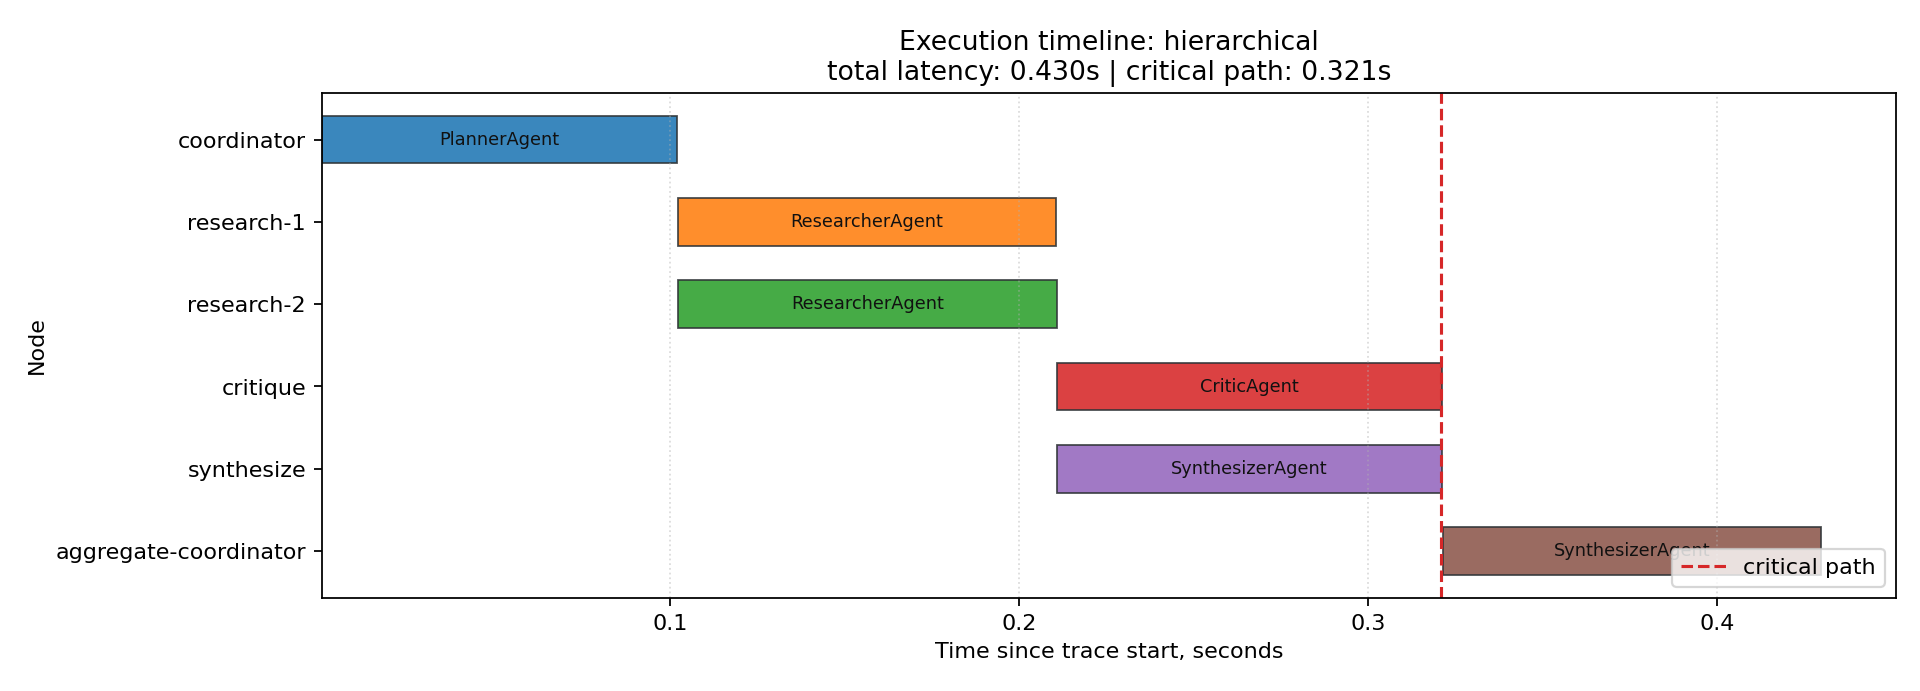
\includegraphics[width=0.86\textwidth]{timeline_execution_trace_hierarchical.png}
\caption{Gantt chart / execution timeline из \code{results/execution\_trace.json}}
\label{fig:timeline}
\end{figure}

\section{Ограничения результатов}

\begin{longtable}{p{0.28\textwidth}p{0.62\textwidth}}
\caption{Ограничения эксперимента}\\
\toprule
Ограничение & Влияние на интерпретацию \\
\midrule
\endfirsthead
\toprule
Ограничение & Влияние на интерпретацию \\
\midrule
\endhead
Mock agents & Latency и results не являются измерениями real LLM API. \\
Synthetic graphs & Scenarios упрощают реальные workflows и dependency patterns. \\
Heuristic quality model & Quality score не измеряет семантическое качество текста. \\
Synthetic failure model & Failure probabilities не откалиброваны на production traces. \\
Learned baseline & Nearest-neighbor selector не является полноценной ML policy. \\
Fixed benchmark configuration & Численные результаты относятся к текущему seed/runs/config и должны пересчитываться при изменениях. \\
\bottomrule
\end{longtable}

\chapter*{Заключение}
\addcontentsline{toc}{chapter}{Заключение}

В ходе работы был реализован и стабилизирован исследовательский прототип адаптивной оркестрации многоагентных LLM-систем на основе DAG. Проект включает DAG model, graph metrics, weighted metrics, topology selectors, executors, mock agents, quality evaluation, failure simulation, robustness metrics, benchmark runner, CLI/config layer, visualizations и tests.

Ключевые улучшения финальной версии:
\begin{enumerate}
  \item cost-aware adaptive selector;
  \item weighted graph metrics и weighted critical path;
  \item learned adaptive selector как lightweight nearest-neighbor baseline;
  \item Gantt chart / execution timeline visualization;
  \item heuristic quality evaluation;
  \item synthetic failure simulation and recovery logic;
  \item unified CLI и experiment configs;
  \item unit tests и reproducibility checks.
\end{enumerate}

По фактическому \code{benchmark\_summary.csv} финальный benchmark сравнил static topologies, rule-based adaptive, cost-aware adaptive и learned adaptive. В текущем запуске learned selector использовал сохранённую модель \code{results/learned\_selector\_model.json}. Полученные результаты показывают, что учет стоимости и critical path помогает выбирать более подходящую topology в synthetic setup, однако работа не утверждает универсальное превосходство какого-либо selector mode.

Основные ограничения остаются следующими: используются mock agents, synthetic graphs, heuristic quality evaluation и synthetic robustness model; learned selector является baseline и требует калибровки на реальных traces.

Future work:
\begin{enumerate}
  \item подключить real LLM backend;
  \item откалибровать cost, overhead и failure model на реальных traces;
  \item развить learned selector до более сложной learned policy;
  \item добавить dynamic re-orchestration во время выполнения DAG;
  \item провести evaluation на реальных задачах и real-world traces.
\end{enumerate}

\appendix
\chapter{Команды воспроизведения}

\begin{lstlisting}
$env:PYTHONDONTWRITEBYTECODE='1'; python -m unittest discover -s tests
python demo.py
python run.py benchmark --runs 1
python run.py train-selector --runs 100 --output results/learned_selector_model.json
python run.py benchmark --selector learned_adaptive --model results/learned_selector_model.json --runs 10
python run.py benchmark --selector all --model results/learned_selector_model.json --runs 10
python run.py visualize --trace results/execution_trace.json
\end{lstlisting}

\chapter{Файлы результатов}

В работе использованы следующие фактические файлы:
\begin{enumerate}
  \item \code{results/benchmark\_results.csv};
  \item \code{results/benchmark\_summary.csv};
  \item \code{results/learned\_selector\_model.json};
  \item \code{results/latency\_comparison.png};
  \item \code{results/topology\_efficiency.png};
  \item \code{results/critical\_path\_impact.png};
  \item \code{results/timeline\_execution\_trace\_hierarchical.png}.
\end{enumerate}

\bibliographystyle{plain}
\bibliography{references}

\end{document}
